\newpage
\section{Kinetic Monte Carlo Setup}
\label{Chap:Al/Vac:section:KMC}

Most parts of the \ac{KMC} algorithm were implemented following the approach we discussed in Chap. \ref{Chap:Mech:KMC}. In this implementation, several points are worth noticing: 1) Event list is determined on the fly. We consider the first nearest neighbor exchange of vacancies. This yields a total of 12 times the total number of vacancies possible events. 2) Then, a \ac{NN} potential is used, instead of traditional empirical potentials or analytical equations, to evaluate diffusion barriers. Noting that all the four symmetry equivalent structures are taken into consideration. 3) At each step, both the forward and backward diffusion barriers of executing the current jump will be calculated to obtain the energy change of the current system, via:
\begin{align}
\Delta E = {E_a}^{forward} - {E_a}^{backward}
\label{Chap:Al/Vac:eq:barrier-EDiff}
\end{align}
where $\Delta E$ is the energy difference between initial and final state, ${E_a}^{forward}, {E_a}^{backward}$ are the forward/backward diffusion barrier, respectively. And the overall energy change as time-evolving is cumulated. 4) In order to boost the system out of low-energy barrier trapping states, a local super-basin method is also implemented based on Ref. \cite{fichthorn2013local}.

For the \ac{KMC} simulations, (30x30x30) supercell containing 108,000 atoms were used. 3240 Mg atoms, 1700 Zn atoms and 1 vacancy atom were randomly chosen among 108,000 atoms. This setup corresponds to $\sim$ 3 atom. \% of Mg, $\sim$ 2 atom. \% of Zn and a vacancy concentration of $\sim$ 1e-6. The probability, $p_k$, of selecting an event $k$ is calculated, via:
\begin{subequations}
\begin{align}
& p_i = r_i / R    \label{Chap:Al/Vac:eq:prob} \\
& r_i = \mu_a * exp(- E_a / k_B T)  \label{Chap:Al/Vac:eq:rate} \\
& R = \sum_{j=1}^N r_j \label{Chap:Al/Vac:eq:R} \\
& \sum_{k=1}^{i-1} p_k < rand < \sum_{k=1}^{i} p_k \label{Chap:Al/Vac:eq:choice}
\end{align}
\end{subequations}
where $\mu_a$ is the diffusion pre-exponential factor, $E_a$ is the diffusion barrier, $k_B$ is the Boltzmann constant, T is the temperature, $N$ is the total number of events, and $rand$ is a random number $\in [0, 1)$. In reality, the diffusion pre-exponential factor, AKA the attempt frequency, and the diffusion barrier depend on the specific configuration \cite{osti_323431,van2001first,le2002kinetic} and type of element which the vacancy jumps to\cite{clouet2004nucleation}. We used \ac{NN} to predict the diffusion barrier, $E_a$, based on local environments. However, the attempt frequency, $\mu_a$, was chosen to use a Debye frequency of 1e13 Hz for all the jump pairs, regardless of their species and local environments. Usually, the pre-exponential factor can results in a 10 times difference. This is still tolerable to predict the event accurately, considering that the difference introduced by the exponential term would be much larger.


\newpage
\begingroup
\begin{figure}[!ht]
  \centering
  \subfigure{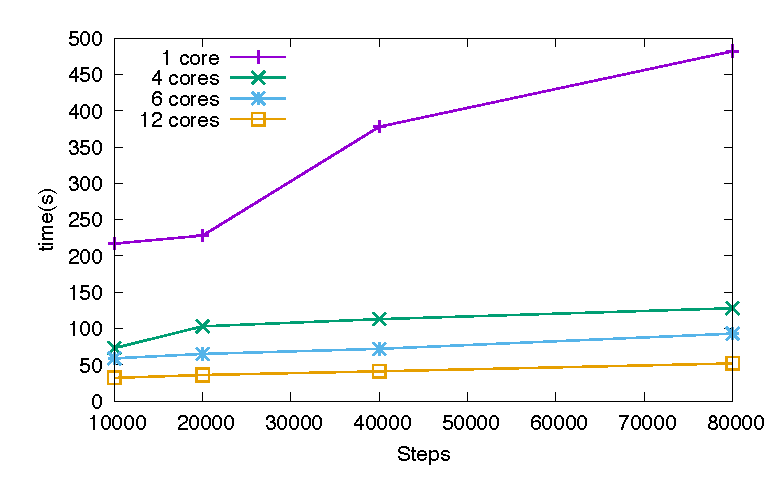
\includegraphics[width=0.75\linewidth]{Chap5/plots/scale.eps}}
\caption[Scalability of KNN2 code on Great Lakes HPC.]{Scalability of KNN2 code for 108,000 atoms on Great Lakes HPC from the University of Michigan with 2x 3.0 GHz Intel Xeon Gold 6154 processors and InfiniBand HDR100 networking, capable of 100 Gb/s throughput.}
\label{Chap:Al/Vac:fig:scale}
\end{figure}
\endgroup


As we mentioned above, all four symmetry equivalent structures needed to be calculated to evaluate diffusion barriers accurately, and both forward and backward diffusion barriers were required. Therefore, a total of 8 calculations were needed for one event. Therefore it becomes important to speed up calculations. We used \ac{MPI} to parallelize our \ac{KMC} simulations. Two parts are benefited significantly from parallelism implementation: 1) building initial neighbor list of every atom; 2) \ac{KMC} events calculation. Note that once the initial neighbor list is built, one can keep updating the neighbor list on the fly. Besides, diffusion barriers and event rates of 12 possible jumping events of one vacancy were distributed to different cores and collected afterward. We tested the scalability of the code, as shown in Fig. \ref{Chap:Al/Vac:fig:scale}. A (30x30x30) supercell containing 108,000 atoms, was used for this testing. Calculations up to 80,000-steps were tested and benchmarked with the usage of different numbers of nodes. For very limited-steps cases, 10,000-steps for example, more cores showed more advantages, as the initial setup of the neighbor list takes a considerable amount of time. As the simulation goes on, the cost of communication between cores does not affect the scalability significantly.